\documentclass[11pt]{article}
\usepackage{fullpage,amsthm,amsfonts,amssymb,epsfig,amsmath,times,amsthm}
\usepackage{tabu} 
\usepackage{pgfplots}

\newtheorem{theorem}{Theorem}
\newtheorem{claim}[theorem]{Claim}
\newcommand\tab{\setlength\parindent{24pt}}

\begin{document}
	
	\begin{center}
		{\bf\Large CMPS 102 --- Fall 2018 --  Homework 3}\\
		Alyssa Melton\\
		I have read and agree to the collaboration policy. \\
		Collaborators: none\\
	\end{center}
	
	%------------------------------------------------------------------------------	
	%------------------------------------------------------------------------------
	
	\section*{Solution to Problem 1}
		We are given a set of days, 1 to \textit{n}. 
		For each corresponding day, we are given the price of the crop. 
		We want to find the maximum amount of profit that Phillip could have made in these \textit{n} days.
		
		While thinking through different things that might help to solve this problem, I graphed prices of crop over \textit{n} days that were given as an example, namely: \\
		\\
		\begin{tabu} to 1 \textwidth { | X[c] | X[c] | X[c] | X[c] | X[c] | X[c] | X[c] | X[c] | X[c] | X[c] | X[c] | X[c] | X[c] | X[c] | X[c] |}
			\hline
			Day & 1 & 2 & 3 & 4 & 5 & 6 & 7 & 8 & 9 & 10 & 11 & 12 & 13 & 14 \\
			\hline
			Price  & 13  & 11 & 8 & 10 & 7 & 12 & 12 & 17 & 14 & 9 & 6 & 8 & 12 & 11  \\
			\hline
		\end{tabu}\\
	\\
	\\
		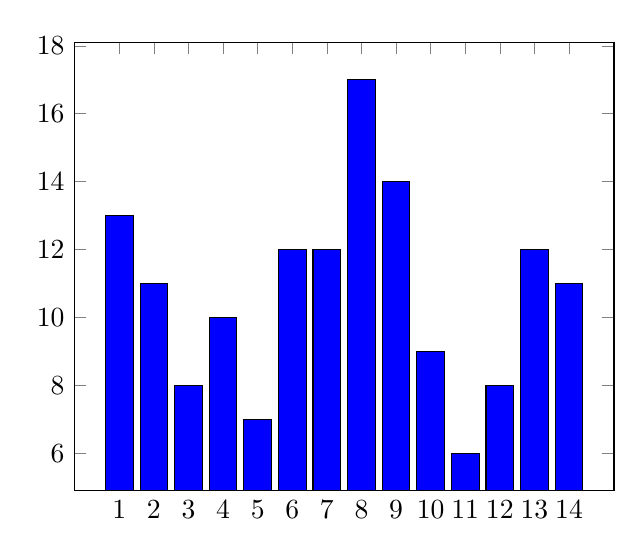
\begin{tikzpicture}
				\begin{axis}[
				symbolic x coords={1, 2, 3, 4, 5, 6, 7, 8, 9, 10, 11, 12, 13, 14},
				xtick=data
				]
				\addplot[ybar,fill=blue] coordinates {
					(1,   13)
					(2,  11)
					(3,   8)
					(4, 10)
					(5, 7)
					(6, 12)
					(7, 12)
					(8, 17)
					(9, 14)
					(10, 9)
					(11, 6)
					(12, 8)
					(13, 12)
					(14, 11)

				};
				\end{axis}
		\end{tikzpicture} \\
		\\
		We are given that the most profit is gained, for this partiuclar example, is by doing the following:\\
		Buy a cart on day 3, sell the cart on day 4, with a margin of 2;\\
		buy a cart on day 5, sell a cart on day 8, with a margin of 10;\\
		buy a cart on day 11, sell a cart on day 13, with a margin of 6.\\
		Now, comparing these values to the graph above, I noticed that these directly correspond with the peaks and valleys of the graph. \\
		\\
		Defintions:\\
		A day's crop price, $price[x]$, is a peak if $price[x] \leq price[x-1]$ and $price[x] \geq A[x+1]$\\
		A day's crop price, $price[x]$, is a valley if $price[x] \geq price[x-1]$ and $price[x] \leq A[x+1]$\\
		\\
		Let us assume that the most profit is gained by buying crop at a price valley, and selling crop at a price peak. Now, consider the following algorithm:\\
		\\
		$profit = 0.\\
		purchase price = null.\\
		profit margin = null.
		price[0] = null.\\
		price[n+1] = null$.\\
		\\
		for each day \textit{i}, 1 to \textit{n}:\\
		\indent  if $price[i-1] \geq price[i]$ and $price[i] \leq price[i+1]$\\
		\indent \indent if $purchase price = null$\\
		\indent \indent \indent buy crop on day \textit{i}.\\
		\indent \indent \indent purchase price = $price[i]$\\
		\indent else if $price[i-1] \leq price[i]$ and $price[i] \geq price[i+1]$\\
		\indent \indent if $purchase price \neq null$ \\
		\indent \indent \indent sell crop on day \textit{i} \\
		\indent \indent \indent $profit margin = price[i] - purchase price$ \\
		\indent \indent \indent $profit = profit + profit margin$ \\
		

	\begin{claim} 
		The most profit is gained by buying crop at a price valley, and selling crop at a price peak. 
	\end{claim}

	\begin{proof}
		If the above algorithm, call it, \textit{Greedy}, is not optimal,
		then there must be some other algorithm, call it \textit{O}, that is optimal. 
		Say that \textit{O} is the same as \textit{Greedy} up until $tie_{k+1}$, and $tie_k$ was the last tie that was the same as the \textit{Greedy}. Then, this tie must have tied two ropes that were not both the smallest ropes in the list, otherwise it would be the same as \textit{greedy}. Call the two smallest ropes $r_1$ and $r_2$. Any other ropes, $r_i$ or $r_j$ where $i, j \in \{1, 2, ... n\}$, is longer than $r_1$ and $r_2$. Then it must be that $r_i + r_j > r_1 + r_2$. Because the cost of adding $r_i$ and $r_j$ is greater than or equal to $r_1 + r_2$, \textit{Greedy} takes no harm in adding $r_1$ and $r_2$ instead. Thus, the \textit{Cost} of \textit{Greedy} must be at most the \textit{Cost} of \textit{O}, thus \textit{Greedy} must be, if not also, optimal. 
	\end{proof}

	\begin{claim} 
	The above algorithm is $O(nlog$ $n)$. 
\end{claim}

\begin{proof}
	The algorithm takes $O(nlog$ $n)$ to sort the list (or build the min-heap).
	It then extracts the top two smallest ropes in $O(log$ $n)$ time, and does this $n$ times, so we get $2*n*logn$.
	It then inserts the new rope back in in O(logn) time and does this $n$ times.
	We ultimately get $nlog$ $n + 2nlog$ $n + nlog$ $n $ which evaluates to $O(nlog$ $n)$
\end{proof}

	\newpage
	
	
\end{document}
